% !TeX spellcheck = en_US
\documentclass[pdftex,english,oribibl]{llncs}

%% Spracheinstellungen laden
\usepackage[english]{babel}

%% Schriftart in der Ausgabe/Eingabe
\usepackage[T1]{fontenc}
\usepackage{textcomp}
\usepackage[utf8]{inputenc}

%% Zitate
\usepackage[numbers]{natbib}
\bibliographystyle{abbrvnat}
%\bibliographystyle{dinat}
%\bibliographystyle{plainnat}
%\bibliographystyle{splncs}
%% Similar to option "sectionbib" but \refname instead of \bibname
\makeatletter
\renewcommand\bibsection{\section*{\refname\@mkboth{\MakeUppercase{\refname}}{\MakeUppercase{\refname}}}}
\makeatother

%% Index
%\usepackage{makeidx}
%\makeindex

%% PDF Einstellungen
% muss nach natbib geladen werden!
\usepackage{nameref}
\usepackage{varioref}
\usepackage[pdfusetitle,pdftex,colorlinks]{hyperref}
\hypersetup{pdfborder={0 0 0}}
\hypersetup{bookmarksdepth=3}
\hypersetup{bookmarksopen=true}
\hypersetup{bookmarksopenlevel=1}
\hypersetup{bookmarksnumbered=true}
\usepackage{color}
\hypersetup{colorlinks=false}

%\usepackage[section]{tocbibind}

\makeatletter
\gdef\@keywords{}
\def\keywords#1{\gdef\@keywords{#1}}
\gdef\@subtitle{}
\def\subtitle#1{\gdef\@subtitle{#1}}

%% modified from llncs
\renewenvironment{abstract}{%
  \list{}{\advance\topsep by0.35cm\relax\small%
          \leftmargin=1cm%
          \labelwidth=\z@%
          \listparindent=\z@%
          \itemindent\listparindent%
          \rightmargin\leftmargin}%
          \item[\hskip\labelsep\bfseries\abstractname]}{%
  \if!\@keywords!\else{\item[~]\item[\hskip\labelsep\bfseries\keywordname]\@keywords}\fi%
  \endlist}

\AtBeginDocument{%
  \if!\@subtitle!\else\hypersetup{pdfsubject={\@subtitle}}\fi
  \if!\@keywords!\else\hypersetup{pdfkeywords={\@keywords}}\fi
}
\makeatother

% llncs hyperref fix
\makeatletter
\providecommand*{\toclevel@author}{0}
\providecommand*{\toclevel@title}{0}
\makeatother

%% Grafiken
\usepackage[pdftex]{graphicx}
\DeclareGraphicsExtensions{.pdf,.jpg,.png}
\usepackage{subfigure}

%% Mathe
\usepackage{amsmath}
\usepackage{amssymb}

%% Listings
\usepackage{listings}
\lstset{escapechar=\%, frame=tb, basicstyle=\footnotesize}

%% Sonstiges
\newcommand{\TODO}[1]{\par\textcolor{red}{#1}\marginpar{\textcolor{red}{TODO}}}
\newcommand{\TODOX}[1]{\textcolor{red}{#1}\marginpar{\textcolor{red}{TODO}}}
\newcommand{\inlineQuote}[1]{''#1``}
\pagestyle{plain}

% Keine "Schusterjungen"
\clubpenalty = 10000
% Keine "Hurenkinder"
\widowpenalty = 10000 \displaywidowpenalty = 10000

%svg and pdf imports
\usepackage{svg}
\usepackage{pdfpages}

%
\usepackage{enumitem}
\usepackage{blindtext}


%tables
\usepackage{tabularx}
\usepackage{booktabs}
\usepackage{multicol}
\usepackage{makecell}

%figure and table caption setup
\usepackage{caption}
\captionsetup{labelfont=bf,format = hang }

%%%%%%%%%%%%%%%%%%%%%%%%%%%%%%%%%%%%%%%%%%%%%%%%%%%%%%%%%%%%%%%%%%%%%%%%%%%%%%%
%%% BEGIN DOCUMENT
%%%%%%%%%%%%%%%%%%%%%%%%%%%%%%%%%%%%%%%%%%%%%%%%%%%%%%%%%%%%%%%%%%%%%%%%%%%%%%%
\title{Learning and Predicting the Performance of Configurable Software Systems}
\subtitle{Seminar - Advanced Software Engineering:\\
Non-Functional Aspects in Software Engineering}
\author{Lion Wagner}
\institute{University of Stuttgart\\Institute of Software Technology (ISTE)\\70569 Stuttgart, Germany}

\newcommand\AFID{\hyperref[sec:AFID]{\textit{AFID}}}
\newcommand\VAPP{\hyperref[sec:VAPP]{\textit{VAPP}}}
\newcommand\WHAT{\hyperref[sec:WHAT]{\textbf{WHAT}}}
\newcommand{\CART}{\hyperref[sec:CART]{\textbf{CART}}}




\begin{document}


\maketitle
\begin{abstract}
  Today's programs are mostly highly configurable and customizable. Popular applications like Apache or MySQL can have hundreds of configurable parameters. Whilst providing flexibility to a customer this also brings some problems as have shown: having so many options can also heavily influence the performance of a software system. And the more options there are, the harder it gets to predict the behavior of software system. This paper will show that a brute force approach to this problem does not work as a general solution. Further it is going to explain and compare four different prediction methods for learning about the performance of highly configurable software systems. Also, the in this context often used machine learning strategy of Classification and Regression Trees is presented. 
\end{abstract}


\section{Introduction} \label{sec:introduction}

As modern programs grow larger and more powerful they also provide many configuration opportunities to their customers. In some cases the number of parameters can be even greater than 500. Examples for this can be found in \cref{fig:paramters}. With this large amounts of configuration options stakeholders or customers can be satisfied easier since they can tailor a program to their specific requirements. But with this large amount of options comes a bigger problem: \inlineQuote{Unpredictability}. Looking at an example of Apache Storm (\cref{fig:ApacheStorma}) shows that the performance of two configurations of a program can differ significantly. \cref{fig:ApacheStormb} shows that solely changing a single parameter can increase the response time of Apache Storm by up to 100\%. Without using prediction methods such results are only visible after executing and measuring multiple, if not all, configurations of a system. Or in other words: when looking only at a single configuration, one cannot conclude whether that configuration is any good for the current requirements in.

This is where prediction comes into play. By learning about the performance of some configurations of the system it tries to generate a function that can give an expected performance for a not measured configuration. This can be used to solve the just mentioned problem of finding a near optimal solution.
Furthermore, performance prediction can be used to find default configurations. These should be configurations that fulfils most requirements to an acceptable level. 
The most straightforward  approach to this problem would be a \textit{brute-force} solution. In this case that would mean measuring each and every single valid configuration. As we will see later in \cref{sec:BruteForce} this approach is in general not feasible since the amount of valid configurations scales exponentially with the number of parameters. For that reason other approaches had to be found and especially the efficient sampling of a configuration space turned out to be a problem \cite{CostEfficientSampling_Gou_Siegmund_2015}.

\begin{figure}[t]
	\centering
	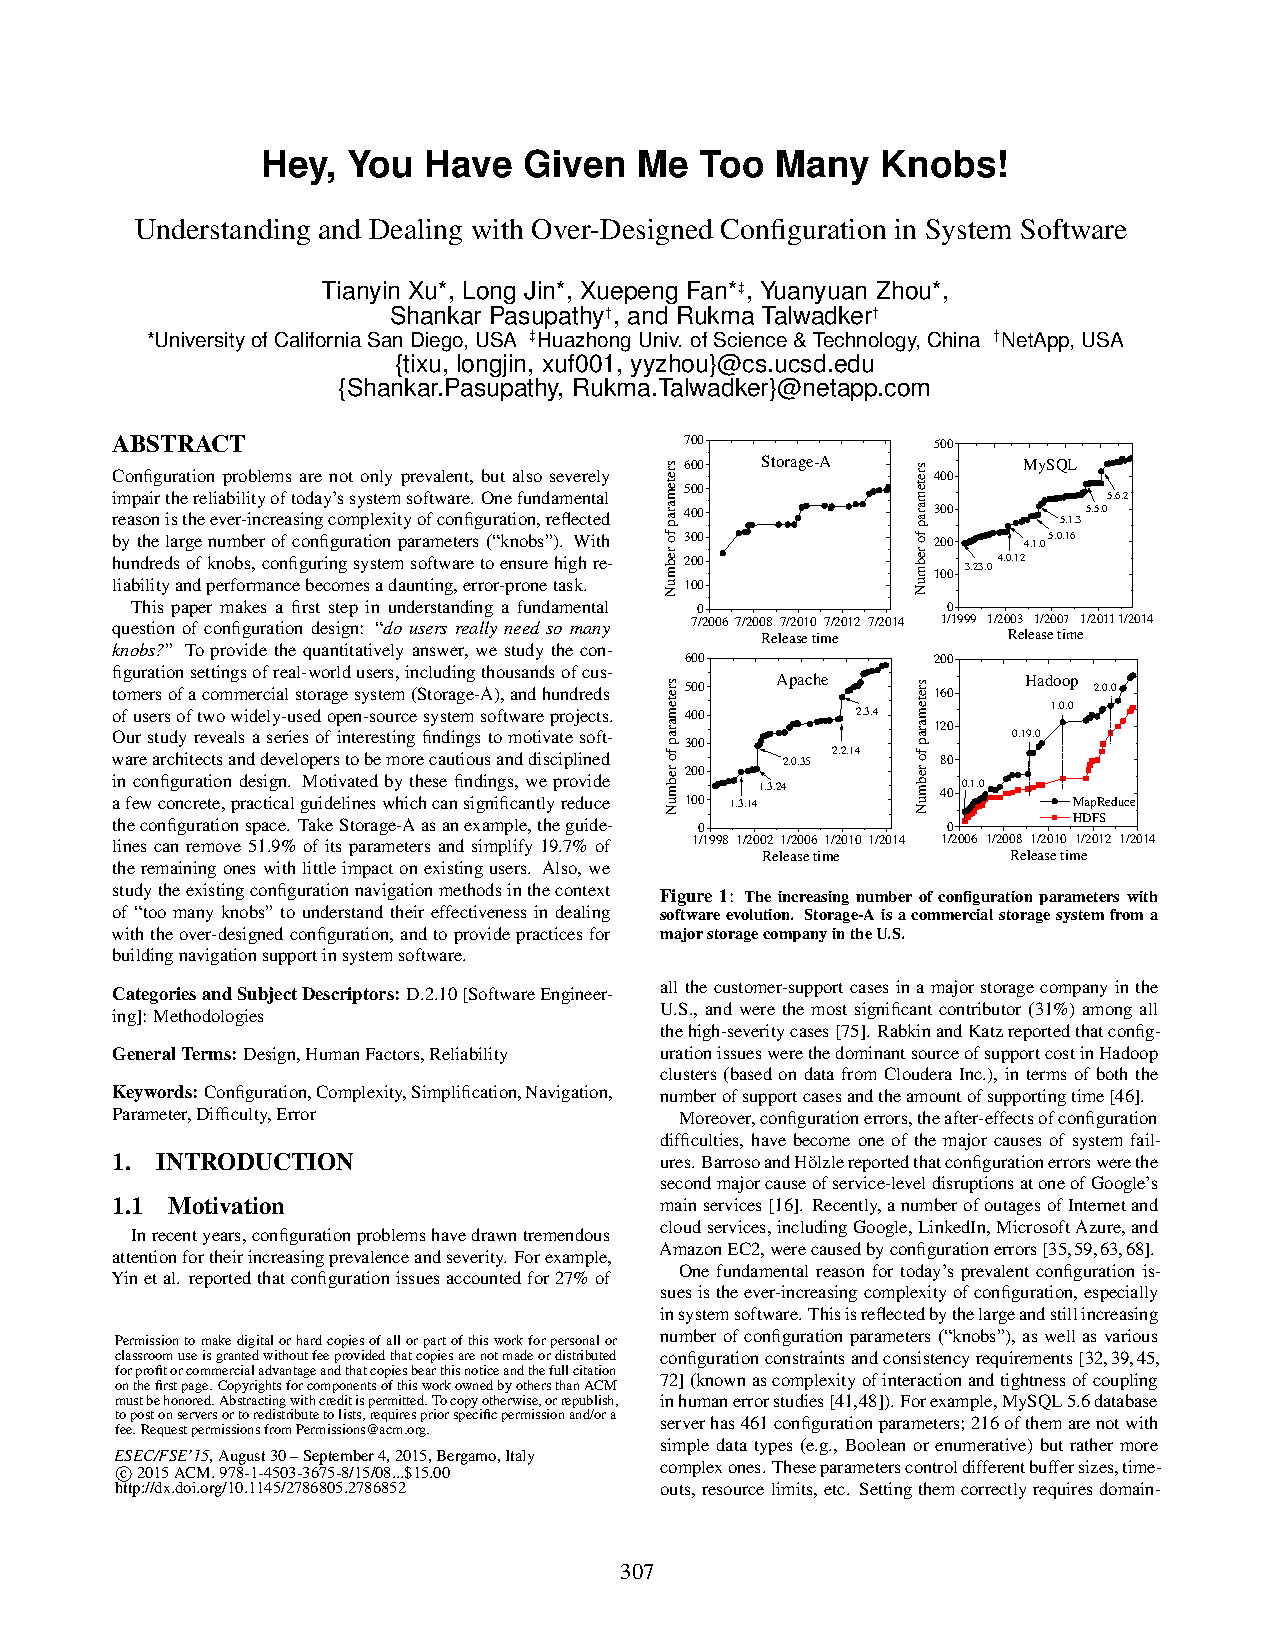
\includegraphics[clip,trim= 11cm 13cm 2cm 7cm]{Paper/thirdParty/HeyYouHaveGivenMeTooManyKnobs.pdf}
	\caption{Number of parameters of different popular programs \cite{YouveGivenMeTooManyKnobs}.}
	\label{fig:paramters}
\end{figure}
\begin{figure}[t]
	\begin{subfigure}{.45\linewidth}
		\centering
		\begin{tikzpicture}
		\node at (0,0)[anchor=north west,inner sep=0] {\includegraphics[page=5,clip,trim=4cm 1cm 8cm 10cm,width=\linewidth] 
		{Paper/thirdParty/vamos_keynote_norbert_siegmund.pdf}};
		\draw [white,fill] (0,0) rectangle (3,-.2); %hide text left on the picture
		\end{tikzpicture}
		\caption{Configurations of Apache Storm sorted by measured throughput.}
		\label{fig:ApacheStorma}
	\end{subfigure}\hspace{.1\linewidth}
	\begin{subfigure}{.45\linewidth}
		\centering
		\includegraphics[page=5,clip,trim=17.4cm 1cm 0cm 10cm,width=.8\linewidth]
		{Paper/thirdParty/vamos_keynote_norbert_siegmund.pdf}
		\caption{Possible influences of only two options on the latency of Apache Storm. }
		\label{fig:ApacheStormb}
	\end{subfigure}
	\caption{Measurements done for Apache Strom which shows that configurations can have a significant influence on the performance of a software system.}
	\label{fig:ApacheStorm}
\end{figure}
This paper will focus on showing different approaches and strategies to predicting the performance of a configurable software system. It will mainly discuss approaches developed by Norbert Siegmund et al. \cite{AutomatedFeatureDetectionSiegmund2012,VariabilityAwarePerformancePredictionJianmeiSigmundApel, CostEfficientSampling_Gou_Siegmund_2015, DistanceBasedSampling2019}. They will be explained and compared. More specifically, this paper will have a look at four different approaches besides \textit{brute-force}.

The first discussed technique is \textit{Automated Feature Interaction Detection} (\AFID) \cite{AutomatedFeatureDetectionSiegmund2012}. The goal of this approach is to assign a performance influence value to each feature and feature interaction. This is done by observing and measuring the behaviour of certain configurations. 
The other 4 approaches make use of a CART Tree as their learning choice but differ in the way they choose their sample.
 
\textit{Variability Aware Performance Prediction} (\VAPP) \cite{VariabilityAwarePerformancePredictionJianmeiSigmundApel} uses random sampling to pick which configurations to compile and measure. 

\WHAT~ \cite{DistanceBasedSampling2019}, tires a more mathematical way to find groups of similar configurations without actually measuring them. For this distance based clustering/sampling is used. 

The last two sampling approaches are proposed in the same paper by \citet{CostEfficientSampling_Gou_Siegmund_2015}. 

\textit{Progressive} and \textit{Projective Sampling} are quite similar, since they both take advantage of the fact, that the general formula behind a learning curve is known. With this knowledge they generate a part of the actual curve and fit a function to it. Based on this function an optimal size for the actual sample set can be calculated. Both methods also take the cost of measurements (resources and accuracy) into consideration.\\
All these approaches can reach accuracies of over 94\% on average in the conducted tests of their corresponding papers. This makes them good enough to be relevant for the topic of this paper. Further their results can be compared straightforwardly since they are all tested on the same set of 6 software systems: Berkeley DB C, Berkeley DB Java, Apache, SQLite, LLVM, x264.

\section{Definitions}

Before the actual approaches are discussed it is important to pinpoint the definitions of terms which are used in this paper.

This paper often uses the terms \inlineQuote{parameters}, (configuration) \inlineQuote{options} or \inlineQuote{features}. These terms are all equivalent and describe ways to adjust and optimize functional and non-functional properties of a software system \cite{DistanceBasedSampling2019}.
One can divide into different types of options. Binary options usually have a value of 0 or 1 and describe the activation of a feature. Non-binary options support a wider range of values. For example this could be a setting for the stack-size allowed for a program. Non-numeric options support the input of text. Those could be paths or other addresses.
The set of all configuration options is denoted as $\mathcal{O}$.

A \textit{configuration} can be defined in multiple different ways. \citet{DistanceBasedSampling2019} define a configuration as a function $c : \mathcal{O} \rightarrow \{0,1\}$. It assigns a 1 to each element of $\mathcal{O}$ that is selected and a 0 to those which are not used. \citet{VariabilityAwarePerformancePredictionJianmeiSigmundApel} and
\citet{FasterDiscoveryofFasterSystemConfigurationsSiegmund2017} have a similar approach. But instead of using a function to describe $c$ they use a vector or an n-tuple over $\mathbb{Z}^+_2(= \{0,1\})$. Each position of those enumerations is associated with exactly one feature. As in \citet{DistanceBasedSampling2019} a 1 indicates an activation of a feature and a 0 means that the feature is not used. These definitions obviously describes binary options only, but can be expanded to support non-binary options by using the co-domain of $\mathbb{N}_0$ instead of $\{0,1\}$.

The \textit{configuration space} describes all valid configurations of a system. It is denoted as $\mathcal{C}$.

A \textit{sample} is the subset of a \textit{configuration space} that contains all configurations that are complied and measured during the process of sampling and learning.

To describe the quality of an approach an \textit{accuracy} metric is often used. The \textit{accuracy} is defined as 1-\textit{fault rate}. And in turn the fault rate (or error rate) is defined as 
\begin{equation}
	\text{fault rate}= \frac{|actual-predicted|}{actual}.
\end{equation} This definition can be found in \cite{FasterDiscoveryofFasterSystemConfigurationsSiegmund2017} and \cite{AutomatedFeatureDetectionSiegmund2012}.

\section{On the Applicability of the Brute Force Approach}
\label{sec:BruteForce}
As mentioned previously: \textit{brute force} measuring is not feasible in most cases \cite{AutomatedFeatureDetectionSiegmund2012}. But what is the actual reason behind this?
Let's have a look at an example first:

In one paper, \citet{AutomatedFeatureDetectionSiegmund2012} measured all valid configurations of multiple programs to analyse the accuracy of \AFID. Berkley DB (C) was one of those programs. It is a database management program for embedded systems. It has 19 features and 2560 valid configuration. In the end, it took approximately 426 hours (= 17.75 days) to measure all these configurations. This value calculates to a time of about 10 minutes per configuration measurement. Considering that Berkeley DB (C) is a comparably small program, this is already a significant amount of time but still a time span that might be acceptable be used to get the perfect results of a \textit{brute force} approach.

This changes once one takes a look at larger programs. Modern applications like Apache or MySQL can have hundreds of configuration parameters \cite{YouveGivenMeTooManyKnobs}. Another example was displayed by \citet{VAMOSConference}: SQLite has 77 features that can produce $3 \cdot 10^{77}$ valid configurations. Unfortunately, there is no evidence how the latter number was calculated. Yet, it can be assumed that at least the scale of this number in regard to the number of features is correct. This will be explained in the next paragraph. Coming back to the example: Assuming measuring (compiling + profiling) one configuration would take 5 minutes, a brute-force approach would take $2.5 \cdot 10^{76}$ hours. Obviously, this is not an acceptable duration.

\begin{wrapfigure}{r}{0.5\textwidth}
	%\setlength\belowcaptionskip{-\baselineskip}
	\includegraphics[width = 0.5\textwidth]{presentation/figures/FeatureModel}
	\captionsetup{width=0.95\linewidth}
	\caption{An example of a feature model.}
	\label{fig:FeatureModel}
\end{wrapfigure}

To find out why \textit{brute-force} does not scale well, a generic look at how many configurations per program are needed to be measured helps. This set of all valid configurations can be written down as a \textit{Feature Model}. An example for this is shown in \cref{fig:FeatureModel}. This \textit{feature model} describes the software system called \inlineQuote{DatabaseSystem}. \textit{Feature Models} can be annotated with further logical expressions to also contain cross-feature constraints. Such can also be seen in the just mentioned example. Each \textit{Feature Model} can also be written down as a logical expression. The atomic variables of this expression are the options of the software system. In this context, a configuration is written down as an assignment of each variable of the expression. The tree in \cref{fig:FeatureModel} is equivalent to the function
\begin{equation*}
	V(C)= \text{Base} \land (\text{Version1.5} \oplus \text{Version2.1}) \land (\text{Version1.5} \Rightarrow \neg \text{DBServer}).%Punkt gehört zum Satz
\end{equation*}
For $V(C)=1$, a configuration is considered \textit{valid}. Otherwise, it is not accepted.
An example configuration could look like this:
\begin{align*}
	\textbf{DEFAULT} =  \{&\text{Base} = 1, \text{Version1.5}=0, \text{Version2.1} = 1, \\
	&\text{DBServer} =0, \text{SearchEngine} =0 \}
\end{align*}
Note that these logical expressions can also be applied to non-binary options. The feature \inlineQuote{Base} of the example could also be expressed as a tertiary value:

\begin{equation*}
	\text{Base} =  \begin{cases}
		0, \text{Not selected}\\
		1, \text{Version1.5 selected}\\
		2, \text{Version2.1 selected}
	\end{cases}
\end{equation*}
In this case, $V(C)$ would look like this:
\begin{equation*}
		V(C)= (\text{Base} \Leftrightarrow 1 \lor \text{Base} \Leftrightarrow 2) \land \big((\text{Base} \Leftrightarrow 1) \Rightarrow \neg \text{DBServer}\big).
\end{equation*}
So it is established that set of valid configurations can be expressed as a logical formula.

In this context the most interesting property of this formula is the scaling of the number of valid configurations in relation to the number of options. Without loss of generality, one can assume that a system only has numeric binary options. This can be done since all other types of options would just increase the overall number of options. However, already looking at binary options gives a satisfying result. Since naturally the total number of possible assignments for a logical expression is exponentially large, the number of valid configurations also lies in the exponential space of $\mathcal{O}(2^{\#options})$. In other words: a \textit{configuration space} that would have to measured for a \textit{brute force} approach would be exponentially large. That is the reason why brute-force does not scale well and more sophisticated methods are need for efficient predictions.




%\section{Software Product Lines Performance Influence}

\TODOX{Intro}
tarditionell präprözessoren oder compiler optionen oder startup optionen

\subsection{Introduction into Software Product Lines}

As mentioned above modern software systems are often highly configurable and customizable. To be able to provide such a large amount of customization, software engineers adopted the concept of \textit{mass customization} inside a product line. A technique mostly known from the automotive industry\cite{SPLEngineering}.\cite{SPLEngineering} further describes how a general product-line functions: There is a \textit{common platform}, which is in itself expandable and holds all basic functionalities. It also provides interfaces for adding on parts (features). Some parts are mandatory and some are optional. For each part there might be different versions or variations that are interchangeable.\\

\begin{figure}%{c}{\textwidth}
	\centering
	\setlength\belowcaptionskip{-\baselineskip}
	\captionsetup{width=0.95\linewidth}
	\includesvg[scale = 0.7]{figures/VisualStudioSPL.svg}
	\caption{Partial view of the Visual Studio Product Line \cite{VisualStudioSPL}. (Assuming a Microsoft is using core libaries for its product. Which is likely since .Net Core runs on all major operating systems.) }
	\label{fig:VSSPL}
\end{figure}\noindent
Software product lines (SPL) inherit this behavior of reusing existing components to enhance the development process \cite{IssuesAndModelsInSPL}. They are used to create a software product that is highly configurable and customizable. Products inside a SPL can even serve as a common platform for further customization. A more detailed look at the economical thought behind SPLs is given by \citet{IssuesAndModelsInSPL}.\\
An example of a SPL would be the Visual Studio product line from Microsoft as shown in \autoref{fig:VSSPL}. The common platform are some core libraries that provide shared code to all products of this line. The products themselves add platform or usage specific features (parts) to the core to offer a broad variation of products. The Visual Studio IDE even splits up further into 3 products that all serve a different purpose, but use same code base. Note that \hyperref[fig:VSSPL]{figure 1} only displays static variations of the product line. Almost all versions are additionally dynamically expendable via plug-ins and customizable via options and preferences.

\subsection{Performance Influences of Feature Binding in SPLs}

The following section is based on Combining Static and Dynamic Feature Binding in Software Product Lines~by~\citet{CombiningStaticandDynamicFeatureBinding}.\\
When designing a SPL one has a choice for each feature to either bind it statically or dynamically.
A statically bound feature is compiled directly into the binary of a program. Its always available to the environment when needed but uses up binary space to do so.
When dynamically binding a feature it is not a part of the core binary, yet a part of an external \textit{feature library}. Once such a feature is needed the core loads the according library from an external source. This leads to the core binary being smaller but the size needed for each feature is increased by some meta-data (size, location, format, etc. of the feature library). Multiple features can be combined into one feature library for optimization. Feature libraries are also called \textit{binding units}. Note that \cite{CombiningStaticandDynamicFeatureBinding} uses the \textit{decorator pattern} for the realization of dynamic feature binding.\\
To describe the effects of binding types we use the terms \textit{functional} and \textit{compositional overhead}. A functional overhead  originates form features (or binding units) that are loaded inside a program yet never used. In turn a compositional overhead is found as meta data that is needed to describe dynamic behavior.\\An abstract example: A program core consisting out of 3 features and uses up~2MB of (hard-drive) memory. We extract 1 feature that is rarely used into a dynamic link library with the size of~1.1MB. Afterwards our core is only~1MB large. We can already conclude that our original program had a functional overhead of~1MB by subtracting the old and the new binary size. When using the extracted feature our program uses up~2.1MB of memory. So we can say that our compositional overhead for extracting the feature is 0.1MB. That is the data needed to describe the location, format, etc. of the feature library.\\
\TODO{daten aus paper einfügen}
\TODO{Fig 18 einbauen}
Coming back to binding types we have the problem of finding an optimal combination of static and dynamic bindings. \citet{CombiningStaticandDynamicFeatureBinding} suggest to prefer static binding if no dynamic extensibility is required and resources are not limited. A full static bound program has no compositional overhead and thus only requires additional (persistent and transient) memory. However programs that are more limited in their resources may need to be designed to minimize the overall overhead. This is basically the same task of finding an optimal configuration of a program. Techniques regarding the analysis and prediction will come up later in the paper \TODOX{reference einfügen}. The compositional overhead of binding units can be predicted partially since feature libaries have a constant size header (e.g. 5KB per Dynamic Link Library \{DLL\}). A general guideline is to avoid a large number and a large size of binding units. Overlapping binding units as well as dynamic splitting and merging of binding units are possible optimizations. \citet{CombiningStaticandDynamicFeatureBinding} also mention that \inlineQuote{[...] there is no optimal size for a binding unit, a domain expert can define binding units per application scenario.}.
\section{Measuring and Predicting the Performance of Highly Configurable Systems}\label{sec:measuring}

By learning about the performance difference of multiple configurations it is possible to predict a program's performance accurately. This means, that not all (possibly exponentially many) configurations need to be measured. Instead, a small sample size should be enough to predict a program's performance. Multiple ways that use different methods have been proposed over time \cite{FasterDiscoveryofFasterSystemConfigurationsSiegmund2017}. This paper will take a look at
\begin{itemize}
	\item \hyperref[sec:AFID]{Automated Feature Interaction Detection} by \citet{AutomatedFeatureDetectionSiegmund2012},
	\item an \hyperref[sec:VAPP]{incremental/statistical learning approach} by \citet{VariabilityAwarePerformancePredictionJianmeiSigmundApel},
	\item \hyperref[sec:WHAT]{\textbf{WHAT}} a spectral learning approach by \citet{FasterDiscoveryofFasterSystemConfigurationsSiegmund2017},
	\item \hyperref[sec:ProjectiveSampling]{Cost efficient sampling by \citet{CostEfficientSampling_Gou_Siegmund_2015}}
\end{itemize}

\subsection{General Approach}

\citet{VariabilityAwarePerformancePredictionJianmeiSigmundApel} defines two problems to be solved by prediction approaches:
\begin{enumerate}
	\item Predicting the performance of a not measured configurations.
	\item Finding a function $f$ that shows the correlation between the properties of measured configurations and their performance value and that makes each predicted performance $f(\x)$ of a configuration $\x$ as close as possible to its actual performance.\\	
	\begin{equation}
	f : \mathcal{C} \rightarrow  \mathbb{R} \text{ such that} \sum_{(\x,y) \in S} L(y,f(\x)) \text{ is minimal}
	\end{equation}\\
	$S$ is a sample and	$L$ is a loss function to penalize errors in prediction. $(\x,y)$ is a pair of a configuration and its measured performance value. The function $f$ is sometimes called the \textit{performance model} of the system.
\end{enumerate}

\noindent
There is a general pattern for the solution of those problems that comes apparent when looking at different prediction approaches. It can be divided into two steps as displayed in \cref{fig:GeneralApproach}.\begin{figure}
	\includegraphics[page=9,clip,trim=4.1cm 5.9cm 3.9cm 19.4cm, width=\textwidth]{presentation/presentation}
	\caption{General pattern of prediction approaches. }
	\label{fig:GeneralApproach}
\end{figure}

The first step is to sample the exponential configuration space. This means finding configurations from which can be learned about the system. This is done by using efficient sampling techniques like spectral sampling \cite{DistanceBasedSampling2019} or progressive sampling \cite{CostEfficientSampling_Gou_Siegmund_2015}.

Once enough and meaningful configurations are found, the learning process starts. Usually the previously chosen configurations are measured, under the condition that this was not already done whilst sampling. The measurement results are fed to a learning process. A lot of different machine learning strategies can be applied \cite{VAMOSConference}. The relative papers typically use \CART's. Based on the found performance model continuing tasks like finding near optimal solutions or in-depth performance analysis can be done \cite{VAMOSConference}.


%\subsection{Approaches to Performance Prediction}\label{sec:approachesPerformanceLearning}

Before looking at actual prediction methods one should have a look at general possibilities for prediction methods. There are 2 general approaches to predicting a component-based system's performance \cite{ComparativeanalysisAbdelaziz112011}. 

\subsubsection[Measurement Approach]{\textnormal{First there is the }measurement-based approach\textnormal{.}} A measurement-based approach uses an analysis tool to monitor an application during execution. Based on the measurements of an existing application a performance model is build and modified. This approach is highly dependent on existing software (e.g.: measured application, analysis tool, operating system). \cite{ComparativeanalysisAbdelaziz112011}

\subsubsection[Model-based Approach]{\textnormal{Secondly there is the }model-based approach\textnormal{.}}
A model-based approach relies on models created by Model Driven Development. It combines multiple models of a system to give a performance prediction. The advantage of this technique is that it does not require a system to exists. Therefore performance modelling can be done before a system is actually composed.
Automation and usage profiles are used to improve the prediction accuracy of this method. Approaches that don't use automation are generally found to be reasoning tools rather than applicable approaches. Some approaches do not consider external factors such as external service calls, usage profiles or the execution environment at all. This decreases the accuracy of their predictions. \cite{ComparativeanalysisAbdelaziz112011}

\subsubsection[Mixed Approaches]{Mixed approaches} are also possible and can occur in many different variations. For example it is possible to parametrize a model based on measured values. \cite{ComparativeanalysisAbdelaziz112011}

This paper will mainly focus on measurement based approaches.%TODO reasoning

%\citet{ComparativeanalysisAbdelaziz112011} also provide an overview over the benefits and disadvantages of each type of approach:





\subsection{Automated Feature Interaction Detection}\label{sec:AFID}

Automated feature interaction detection (AFID) is a measurement-based approach to predicting the performance of a highly configurable system.
It was developed by \citet{AutomatedFeatureDetectionSiegmund2012}. Unlike other methods it does not depend on machine learning but rather tires to directly identify the performance impact of each feature or a combination of features. This method reached a precision of up to 95\% in the experiment conducted by  \citet{AutomatedFeatureDetectionSiegmund2012}.

\subsubsection[Formulars]{\textnormal{Some} Formulars} are needed to descibe a Softwaresystem for AFID .
The composition of using two (or more) units/features is denoted by $\cdot$ . This composition is also called a configuration \cite{VariabilityAwarePerformancePredictionJianmeiSigmundApel}.\\
The interaction of two features is denoted by $a\#b$. By combining both we get a feature interaction:
\begin{equation}
 a \times b = a\#b \cdot a \cdot b
\end{equation} 
This equation expresses, that when using both $a$ and $b$ we also need to consider their interaction $a\# b$. Note that either $a$ or $b$ can also be a configuration.\\
Further Sigmund uses an abstract performance function $\Pi$ that is used to represent some performance value of a configuration:
\begin{align}
\Pi(a \cdot b) &= \Pi(a) + \Pi(b)\label{eq:featureInteraction_SimplePerformance}\\
\Pi(a\#b) &= \Pi(a \times b) - (\Pi(a) + \Pi(b))\\
\Pi(a \times b) &=  \Pi(a\#b) + (\Pi(a) + \Pi(b))\label{eq:featureInteraction_InteractionPerformances}
\end{align}
Following that the performance of a program $P = a \times b \times c$ can be written down as
\begin{equation}\label{eq:featureInteraction_ProgrammPerformance}
\Pi(P) = \Pi(a) +  \Pi(b) +  \Pi(c) +  \Pi(a\#b) +  \Pi(a\#c) +  \Pi(b\#c) +  \Pi(a\#b\#c). 
\end{equation}
The Problem with the equations \ref{eq:featureInteraction_SimplePerformance}-\ref{eq:featureInteraction_ProgrammPerformance} is that they assumes that we can measure the performance of a feature in isolation. This is in general not possible \cite{AutomatedFeatureDetectionSiegmund2012}. Also we are still in the space of $\mathcal{O}(2^n)$ of possible configurations that we need to measure.  
To reduce this Sigmund et al. uses a interaction \textit{delta}. 
\begin{equation}
\begin{split}
\Delta a_C &= \Pi(C\times a) - \Pi(C)\\
&=\Pi(a\# C) + \Pi(a)
\end{split}
\end{equation}
Where $C$ is a base configuration. This formula describes how the performance influence ($\Delta$) of $a$ on a configuration $C$ can be calculated. Its either the performance difference between using $C$ with and without $a$, or the performance influence of $a$ itself plus the influence of the interaction between $C$ and $a$.\\
As a general approach to reduce its search space AFID looks at:\\
\begin{minipage}{\textwidth}
\begin{equation}
	\Delta a_{min} = \Pi(a \times min(a)) - \Pi(min(a))
\end{equation}
\begin{center}
	and
\end{center}
\begin{equation}
	\Delta a_{max} = \Pi(a \times max(a)) - \Pi(max(a))
\end{equation}
\end{minipage}\\[0.3cm]
 Where $min(a)$ is a valid minimal configuration not containing $a$ but to which $a$ can be added to create another valid configuration. $max(a)$ is a valid maximal configuration not containing $a$ but to which $a$ can be added to create another valid configuration.\\
 \subsubsection[Automated Feature Interaction Detection]{\textnormal{For} AFID} 
one first needs to define when a feature is interacting. For this \citet{AutomatedFeatureDetectionSiegmund2012} use the definition of 
 \begin{equation}
 a \text{ interacts} \Leftrightarrow \exists C,D | C \neq D  \land	 \Delta a_C \neq \Delta a_D .
 \end{equation}
 $C~=~min(a)$ and $D~=~max(a)$ are chosen to find interacting features and to reduce the search space for $C$ or $D$ from $\mathcal{O}(2^n)$ to $\mathcal{O}(n)$. By measuring $\Delta a_{min(a)}=\Delta a_C$ and $\Delta a_{max(a)}=\Delta a_D$ for each feature some first information about their behavior can be obtained. If both values for a feature $a$ are similar it does not interact with the features of $max(a)\backslash min(a)$. Otherwise $a$ is marked as interacting. In both cases it can still interact with the features of $min(a)$. In total 4 measurements per feature are required ($\Pi(a \times min(a))$, $\Pi(min(a))$, $\Pi(a\times max(a))$, $\Pi(max(a))$)\cite{AutomatedFeatureDetectionSiegmund2012}.\\
 Since most of the interacting features are known by now one can look for the groups of features whose interaction does have an influence on performance. Again the problem arises that there is an exponential number of possible combinations. Three heuristics are used to simplify the finding of these groups.
 
 \newcommand{\oitem}[2]{{\item[{\parbox[t][0pt][t]{\leftmargin}{\raggedleft #1}}] {\parbox[t]{\textwidth-\leftmargin}{#2}}}}
 \begin{itemize}[leftmargin=4cm]
 	\setlength\itemsep{1em}
 	\oitem{Pair-Wise~Heuristik (PW):\label{lab:PW}}{ Most groups of interacting features appear in the size of two\cite{AutomatedFeatureDetectionSiegmund2012,AnalysisOfTheVariabilityInFortyPreprocessor_BasedSPLLiebig}. So it makes sense to look for pair interaction first.}
 	\oitem{Higher-Order Interactions Heuristic (HO):\label{lab:HO}}{
 		\citet{AutomatedFeatureDetectionSiegmund2012} only look at higher order interactions of the rank of three. More on this later.
 	}
 	\oitem{Hot-Spot Features (HS):\label{lab:HS}}{
 		Based on \cite{FeatureCohesioninSPL, CanWeAvoidHighCoupling?} \citet{AutomatedFeatureDetectionSiegmund2012} assume that hot spot features exist. \inlineQuote{[...] There are usually a few features that interact with	many features and there are many features that interact only with few features.}, these features are the hot spot features.
 	}
 \end{itemize}
Using a SAT-Solver an implication graph as seen in \autoref{fig:ImplicationTree} is generated. Each implication chain in this tree should have at least one interacting feature. When analysing the tree each chain is walked from the top down. The three heuristics will be applied in the order of PW $\rightarrow$ HO $\rightarrow$HS.  

\begin{wrapfigure}{l}{0.5\textwidth}
%\setlength\belowcaptionskip{-\baselineskip}
\includesvg[width = 0.5\textwidth]{figures/ImplicationTree}
\captionsetup{width=0.95\linewidth}
\caption{Implication tree example found in \cite{AutomatedFeatureDetectionSiegmund2012} }
\label{fig:ImplicationTree}
\end{wrapfigure}

First the influence of every feature on another chain is measured (\hyperref[lab:PW]{PW-heuristic}). In the example of \autoref{fig:ImplicationTree} the interactions would be measured in this order:\inlineQuote{$F1\#F6, F1\#F7, F4\#F6,\\ F4\#F7, F6\#F11,F7\#F11,F1\#F11,\\ F4\#F11$}\cite{AutomatedFeatureDetectionSiegmund2012}. If an interaction impact $\Delta a\#b_C$ exceeds a threshold it is recorded.

Secondly, the \hyperref[lab:HO]{higher order interaction heuristic} is applied. Higher order interactions can be relatively easily found by looking hat the results of the PW-Heuristik. Three features that interact pair-wise are likely to interact in a third order interaction. For example, looking at features $a$, $b$ and $c$- If $\Delta a\#b_{C1}$ and $\Delta b\#c_{C2}$ have been recorded $\{a\#b, b\#c, a\#c\}$ all have to be non zero to find a third order interaction. Interactions with and order higher than three are not considered to prevent too many measurements.

Lastly Hot-Spot features are detected (\hyperref[lab:HS]{HS-heuristic}). This is done by counting the interactions per feature. If the number of interactions of a feature is above a certain threshold (e.g. the arithmetic mean) it is categorized as a Hot-Spot feature. Based on the hotspot features further third order interactions are explored. Again higher order interactions are not considered to prevent too many measurements. \\
After applying the three heuristics all detected interacting features or feature combinations are assigned a $\Delta$ to represent their performance influence on the program.

\begin{wrapfigure}{r}{.5\textwidth}
	\centering
	\setlength\belowcaptionskip{-2\baselineskip}
	\captionof{table}{Results of average accurcy found by \citet{AutomatedFeatureDetectionSiegmund2012}}
	\label{tab:avgAccuracy}
	\begin{tabular}{c|c}
		Approach&avg. Accuracy\\\midrule[1pt]
		FW&79.7\%\\\hline
		PW&91\%\\\hline
		HO&93.7\%\\\hline
		HS&95.4\%\\\hline
	\end{tabular}
\end{wrapfigure}\noindent
\citet{AutomatedFeatureDetectionSiegmund2012} tested AFID on six different SPLs (Berkely DB C,Berkely DB Java, Apache, SQLite, LLVM, x264). Each program was tested under four approaches: Feature-Wise, Pair-Wise, Higher-Order, Hot-Spot (in this order). Each approach also used the data found by the previous one. Accordingly the results get better the more heuristics are used as seen in \cref{tab:avgAccuracy}. Using only the FW approach means that interactions (and the heuristics) are not considered, yet the accuracy is already at about 80\% on average. A significant improvement can be made by using the PW heuristic. It uses on average 8.5 times more measurements than the FW approach but improves the accuracy to 91\%. Using the HO or HS approach improves the accuracy further by about 2-4\%. However for Apache using the HO over the PW approach even deteriorated the average result by 3.9\% and doubled the standard variation. As already mentioned using the HS approach gives the best accuracy this is true for all 6 tested applications. \citet{AutomatedFeatureDetectionSiegmund2012} also notes that analysing SQLite only needed about 0.1\% of all possible configurations. This hints to the good scalability of AFID.

\subsection{Classification and Regression Trees}
\label{sec:CART}
The next 3 approaches all use a specific type of machine learning strategy to construct their predictors. This method is call Classification and Regression Tree's (\CART). These trees are typically binary trees that divide the given data points into small enough groups so a direct local prediction can be done.
These local prediction are than combined into a global predictor \cite{VariabilityAwarePerformancePredictionJianmeiSigmundApel}. In the context of configurable software systems each point consists at least out of a configuration and an associated performance score. These data point are then fed into the algorithm seen in \cref{alg:CART}.
\begin{figure}[h]
	\lstset{
		mathescape,
		breaklines=true,
	}
	\begin{lstlisting}
1. Start at the root node. Assign all configurations to it.
2. For each option, find the set of options $X$ that minizes the sum of the node impurities in the two child nodes. Divide the configurations assigned to the current node based on $X$ into two disjoint sets and assign those to the corresponding child nodes.
3. If a stopping criterion is reached, exit. Otherwise, apply step 2 and 3 to each child node inturn.
	\end{lstlisting}
	\captionof{lstlisting}{Pseudocode for generating a \CART. Adopted from \citet{ClassificationAndRegressionTrees} to fit software configurations.}
	\label{alg:CART}
\end{figure}
The node impurity is typically calculated by the square mean error. As a stopping criteria the size of the leaf node is used \cite{VariabilityAwarePerformancePredictionJianmeiSigmundApel}. The size of the predictor variables set $X$ is usually 1.
\begin{figure}[h]
	\centering
	\includegraphics[page=4,clip,trim=3.5cm 18cm 3.5cm 1.5cm, width=\linewidth]
	{Paper/VariabilityAwarePerformancePredictionAStatisticalLearningApproach.pdf}
	\caption{Example performance model of X264 generated by CART based on the random sampling, using minimization of the sum of squared error loss \cite{VariabilityAwarePerformancePredictionJianmeiSigmundApel}.}	
	\label{fig:VAPPExampleTree}	
\end{figure}


\subsection{Variability aware Performance Prediction}\label{sec:VAPP}

Variability aware Performance Prediction (\VAPP) is a statistics based approach to performance prediction. With the help of random sampling and \CART s a simple yet effective predictor can be build. The following section is based upon \citet{VariabilityAwarePerformancePredictionJianmeiSigmundApel}. In their own tests \citet{VariabilityAwarePerformancePredictionJianmeiSigmundApel} reached an average precision of 94\% whilst using a sample as large as the ones \AFID~would be using under the PW-heuristic. Further, tests conducted by \citet{FasterDiscoveryofFasterSystemConfigurationsSiegmund2017} with the same sample size showed an accuracy of 92.4\%.\\
\setlength\intextsep{\baselineskip}
\begin{wrapfigure}[12]{R}{.5\linewidth}
	\includegraphics[page=3,clip,trim=11cm 13.5cm 1.5cm 10.25cm, width=\linewidth ]{Paper/VariabilityAwarePerformancePredictionAStatisticalLearningApproach}
	\caption{Overview of the Approach of Variability aware Performance Prediction \cite{VariabilityAwarePerformancePredictionJianmeiSigmundApel}.}
	\label{fig:VAPPOverview}
\end{wrapfigure}
The basic idea of variability aware performance prediction is shown in \cref{fig:VAPPOverview}.
Two cycles can be found:	
\FloatBarrier 
\begin{itemize}	
	\item[$\circ$] The first cycle is outside of the dashed box and describes the basic input-output behavior of a predictor. A user configures a new configuration $\x$ for System $A$ and asks the predictor (dashed box) for a prediction. It replies with a quantitative prediction for $\x$'s performance.
	\item[$\circ$]  In the second cycle a actual prediction is generated based on decision rules which themselves are in turn created by simplifying a performance model (a \CART). Random sampling is used to learn the performance model.
\end{itemize}
Like other approaches, the target of variability aware performance prediction is to get accurate predictions whilst only using a small sample for the creation of the performance model. Nonetheless, \VAPP~offers a free choice of the sample size. The configurations of the sample are chosen randomly out of $\mathcal{C}$. 

\VAPP~uses the tuple-based definition of a configuration. It further defines that each configuration $c_j \in \mathcal{C}$ has an actual performance value $y_j$. For formal correctness it is assumed that every option of a configuration actually influences the performance of the system. Otherwise, a \CART~could not be applied.

In the used \CART~each sub-tree is also called a segment $S_i$, where $i$ determines the location of the sub-tree. This is also shown in \cref{fig:VAPPExampleTree}.\\
For the \textit{local model} $\ell$ of the used \CART~\citet{VariabilityAwarePerformancePredictionJianmeiSigmundApel} choose the arithmetic average:
\begin{equation}
	\ell_{S_i} = \frac{1}{|S_i|} \sum_{y_j \in S_i} y_j
\end{equation}
As a loss function to penalize the prediction errors (node impurity) the sum of squared error loss is selected.
\begin{equation}
	\sum_{y_j \in S_i} L(y_j,\ell_{S_i}) = \sum_{y_j \in S_i} (y_j - \ell_{S_i})^2
\end{equation}
Therefore the best split for a segment $S_i$ is found when
\begin{equation*}
\sum_{y_j \in S_{iL}} L(y_j,\ell_{S_{iL}}) + \sum_{y_j \in S_{iR}} L(y_i,\ell_{S_{iR}})
\end{equation*}
is minimal.

Assuming there are $q$ leafs in a tree than the predictor function $f(\mathrm{x})$ is defined as:
\begin{equation}\textsl{}
f(\mathrm{x})=\sum_{i=1}^{q} \ell_{S_i}I(\mathrm{x}\in S_i)
\end{equation}
where $I$ is an indicator function to indicate whether $\mathrm{x}$ belongs to a leaf $S_i$.\\
For the example of \cref{fig:VAPPExampleTree}, $f(\mathrm{x})$ unwraps to:
\begin{align*}
f(x) = 255&* I(x_{14}=1,x_7=0)\\[-0.1cm]
	 + 268&* I(x_{14}=1,x_7=1)\\[-0.1cm]
	 + 402&* I(x_{14}=0,x_{15}=1,x_3=0)\\[-0.1cm]
	 + 508&* I(x_{14}=0,x_{15}=1,x_3=1)\\[-0.1cm]
	 + 571&* I(x_{14}=0,x_{15}=0,x_3=1)\\[-0.1cm]
	 + 626&* I(x_{14}=0,x_{15}=0,x_3=0)
\end{align*}
Every possible configuration $\mathrm{x}$ is associated with a leaf of the tree. Therefore, $f(\mathrm{x})$ can always be applied.\\

For their Experiment \citet{VariabilityAwarePerformancePredictionJianmeiSigmundApel} test the same software systems as \citet{AutomatedFeatureDetectionSiegmund2012} (\cref{sec:AFID}). They also compared their prediction results with the results produced by \AFID.\\
Since unlike \AFID~the size of a sample for \VAPP~can be chosen freely, some comparable sample sizes were chosen. \citet{VariabilityAwarePerformancePredictionJianmeiSigmundApel} use 4 different sample sizes based on the size of the tested programs. For a program with $N$ features they use samples the size of $N,2N,3N \text{ and } M$. $M$ is the amount of configurations measured by \AFID~using the \hyperref[lab:PW]{PW-heuristic}.
It was found, that the prediction accuracy increases linear with the size of a sample. For a small sample with the size of $N$ the prediction accuracy was at above 92\% in 3 cases. However, for Berkeley DB (C) the prediction accuracy with an $N$ sized samples was at 112.4\% with a standard deviation of $\pm$354.6\%. This shows that \VAPP~is not generally applicable for small samples.
Using a sample size of $M$ significantly improves the average prediction accuracy to a stable average of 93.8\%.\\

\subsection{WHAT}\label{sec:WHAT}
\newcommand{\WHAT}{WHAT}

\WHAT~is a spectral learning approach developt by \citet{FasterDiscoveryofFasterSystemConfigurationsSiegmund2017}. It aims to find an accurate and stable performance model with fewer samples than the previous methods. To reach this goal it uses spectral and regression tree learning. The idea behind spectral learning is mathematical concept of \textit{eigenvalues/-vectors} of a distance matrix between configurations. This has the advantage of automatic noise reduction as \citet{FasterDiscoveryofFasterSystemConfigurationsSiegmund2017} explain: \inlineQuote{When data sets have many irrelevancies or closely associated data parameters $d$, then only a few eigenvectors $e, e\ll d$ are required to characterize the data.}\\
The main advantage of this approach are a reduced sample size needed and a lower standard deviation compared to previously shown methods \cite{FasterDiscoveryofFasterSystemConfigurationsSiegmund2017}.
\citet{FasterDiscoveryofFasterSystemConfigurationsSiegmund2017} divide \WHAT~into 3 parts.\\

\textbf{1. Spectral Learning}

This first step is used to cluster all valid configurations. Every configuration is an element of the feature space $F$. This section uses the same definition for a \textit{configuration} as \cref{sec:VAPPMethods} \footnote{This definition can also be expanded to cover non binary options like a programs stack size. For this $x_i\in\mathbb{R}$ has to be chosen.}. As each configuration is an n-dimensional vector (or n-tupel) it can be placed in an n-dimensional space.\\
\WHAT~gets $N$ different valid configurations as input and is picks a random configuration $N_i$ and two configurations $West$ and  $East$. $West$ is the configuration that is most different to $N_i$ and $East$ is the configuration most different to $West$. In mathematical terms 'most diffrent' means most farthest away. After that a straight through $East$ and $West$ is calculated and all configuration are dived into two cluster by their distance to this line. This process is recursively repeated for each sub-cluster until they reach a threshold size. \citet{FasterDiscoveryofFasterSystemConfigurationsSiegmund2017} use the $\sqrt{|N|}$ as their termination value. We end up with leaf clusters that contain configurations which are similar in their chosen feature options. This process runs in linear time\cite{FasterDiscoveryofFasterSystemConfigurationsSiegmund2017}.\\

\textbf{2. Spectral Sampling}

For the actual sampling a probabilistic strategy is applied: One configuration randomly picked from each leaf cluster is compiled and executed.\\
There are also two other sampling strategies mentioned that will get outperformed by the probabilistic strategy.\\

\textbf{3. Regression-Tree Learning}

This step is similar to \cref{sec:VAPPMethods}. A CART is build from the chosen samples. This time the best split is defined as reaching the minimum of $\frac{A}{N}\sigma_1+\frac{B}{N}\sigma_2$$^,$\footnote{The paper (\cite{FasterDiscoveryofFasterSystemConfigurationsSiegmund2017}) defines $A$ and $B$ as sets and $N$ as a (natural) number. So it may is to assume that the formular actually should be $\frac{|A|}{N}\sigma_1+\frac{|B|}{N}\sigma_2$. This does make sense since this formula weights both standard deviations $\sigma$ proportional to $N$.}. From this CART decision rules can be derived.

\subsubsection{Results} of testing \WHAT~on the programs we introduced earlier show that it has an average precision of 93.4\%. Also the standard deviation is comparably low.\cite{FasterDiscoveryofFasterSystemConfigurationsSiegmund2017}


%The test also show that for a low number of features a Brute-Force (BF) approach might also be viable. Measuring all configurations of Apache took about 213h where as the HS approach took 159h. BF guarantees a 100\% correct prediction where as the HS approach only had 94.7\% accuracy. Its is also worth noting that these tests were done on computers that are (from today's point of view) fairly slow \cite{CPUDatabase}. 

%Performance problems occuring after a while are not covered or predictable by these solutions. They go back to the old Holding problem

% !TeX spellcheck = en_US
\section{Comparison}
\begin{figure}[t]
	\centering
	\captionof{table}{Measureing results of \citet{FasterDiscoveryofFasterSystemConfigurationsSiegmund2017} when comparing the methods of, \AFID(Siegmund), \VAPP(Gou), \WHAT~and projective sampling in combination with CARTs (Sarkar). The \textit{Rank} column is computed using Scott-Knott, bootstrap 95\% confidence, and A12 test \cite{FasterDiscoveryofFasterSystemConfigurationsSiegmund2017}.}
	\label{tab:ConclusionPerformanceOverview}
	\vspace{-.5\baselineskip}
	\includegraphics[page=19, clip=true, trim=2.5cm 13.8cm 6.8cm 3.1cm, width=.9\linewidth]{"Paper/Faster Discovery of Faster System Configurations with Spectral Learning".pdf}
	\vspace{-1\baselineskip}	
\end{figure}
\cref{tab:ConclusionPerformanceOverview} displays the results of an experiment conducted by \citet{FasterDiscoveryofFasterSystemConfigurationsSiegmund2017}, to compare the different prediction methods. The table shows some characteristic properties of each approach.

Siegmund's approach of \AFID~was ranked last on 4 occasions. Its accuracy and standard deviation are the worst in most cases. It mostly ranks lower than \VAPP~whilst utilizing same sample size (Guo(PW)). \WHAT~is the oldest of the presented approaches and its low ranking can be seen as a demonstration on how prediction algorithms evolved over time.

Both versions of \VAPP~appear inconsistently with regard to their rank. Gou(PW) ranks lower than Gou(2N) in half of the six occasions. Generally the version which used a larger sample had a slightly better accuracy, but also suffered from a larger standard deviation. The results show that \VAPP's predictions might not be consistent for not sufficiently large enough samples. This could be attributed to the complete randomness of configuration picking.

Sarkar's approach of using cost-efficient sampling in combination with CARTs ranked best in four out of the six cases. In the remaining two cases it still had an acceptable accuracy. But this consistent high accuracy comes with the cost of using larger samples then other methods. In the case of SQLite, the optimized sample size was 15 times larger than the sample of the next best approach \WHAT. 

Considering all tests \WHAT~had an average standard deviation of only 2.98\%. Having such a low standard deviation was the main goal of \WHAT. When comparing it to other methods, it consistently has a below average standard deviation and an above average accuracy whilst using a smaller sample. Since \WHAT~is also the most recent approach, this further confirms the progress that was made in recent years.

\FloatBarrier
\section{Continuing, Related and Future Work}

This paper covered different types of prediction approaches developed by N. Siegmund et al.\\Many other techniques can be found that are related or used for performance prediction of configurable software systems. Some notable continuing techniques are:
\begin{itemize}[leftmargin=*,align=left]
	\item[\textbf{T-Wise Sampling}] picks configurations that contain every combination of T different features to ensure a diverse sample \cite{T-WiseSampling}.	
	\item[\textbf{Fourier Learning}] theoretically guarantees a accuracy level whilst using a minimal sample. It is based on the Fourier transform and was developed by \citet{FourierLearning}.
	\item[\textbf{Transfer Learning}] uses prediction models that are generated based on simulations of the observed system. These models then get transferred to a predictor of the real system to improve its predictions \cite{TransferLearningforImprovingModelPredictionsJamshidiVKSK17}.	
\end{itemize}

\noindent
As shown, a lot of different prediction approaches with satisfying accuracies are available. To further improve them \citet{FasterDiscoveryofFasterSystemConfigurationsSiegmund2017} propose two different starting points:
 \begin{itemize}
 	 \item  All presented approaches consider all features as equally important. But in some systems a certain option might has a higher priority than others. Hence, weighting techniques for features could improve prediction results.
 	 \item Currently, the sizes of samples are mostly picked manually. This can lead to problems with adaptability and scalability. A future field of research would be the integration of a dynamic progressive sampling techniques, as replacement for the typically used static sample size.
 \end{itemize}

Furthermore, \citet{PerformanceInflunceModels_Sigmund_2015} note that finding valid configurations, for binary and non-binary options is still a problem with exponential complexity. Improvements on related algorithms would lead to a faster discovery of the \textit{configuration space}, test and training sets.

Most approaches concentrate on binary and numeric options only. \citet{PerformanceInflunceModels_Sigmund_2015} show that both can be integrated smoothly, into a prediction approach. However, non-numeric options like paths are not mentioned much in the literature. For example, a database-path can arguably have a huge impact on the performance of a software system. The extension or development of techniques that support non-numeric option could improve predictions for more complex software systems that depend on those kinds of options.

\section{Conclusion}

There are many techniques for learning and predicting the performance of a configurable software system. This paper had a look at different approaches developed by N. Siegmund et al. It was quickly determined that, if enough time and resources are available or a program is sufficiently small, \textit{brute force} can be applied to get perfect prediction results. But since \textit{brute force} does not scale well, more sophisticated methods were developed. Most of those methods produce acceptable results with over 90\% accuracy in many cases. But there is no best approach. Each technique has its own advantages and disadvantages that make it unique. \AFID~has well explainable results, \VAPP~is easy to implement, \WHAT~has a very low standard deviation and when using cost-efficient sampling extremely accurate predictions are possible. Which method a predictor should use is always a question of finding a balance between the possible size of the sample, the targeted accuracy and the applicability of the approach on the current system.



\bibliography{PredictingAndLearningPerformanceOfHighlyConfigurableSystemsBib}
\end{document}
